\section{Task Taxonomy on DOI Timeline Visualization}

In this section, we define an exhaustive set of 31 tasks possible on  DOI Visualization. The tasks are inspired from Shneiderman's data type taxonomy~\cite{shneiderman1996eyes} and Amar et al.'s low-level visual analytic tasks~\cite{amar2005low}. We classify each of 31 tasks into six categories which we propose. Our proposed categories are in context of a eye-tracking user study scenario. 
\begin{itemize}
	\item \textbf{Low level data retrieval:} Tasks under this category encompass with eye-registering of DOI using eye-tracker, simple calculation such as counting, and obtaining the time of a particular event. E.g. Given a list of actors, which of them were viewed at time $t$?
	\item \textbf{Operating with a DOIs identity:} Tasks under this category deals identity of a DOI. E.g. Which movie has user $X$ viewed for longest time?
	\item \textbf{Operating with continuously valued attributes:} Tasks dealing with calculations such as finding maximums, averages, estimating distributions over continuous valued attributes of DOIs fall under this category. E.g. Find the age distribution of actors viewed in time $t_1$ and $t_2$.
	\item \textbf{Operating with discrete valued attributes:} Tasks dealing with calculations  over discrete valued attributes of DOIs fall under this category. E.g. Which user looked at most female actors?
	\item \textbf{Transitions:} Tasks consisting transitions or changing eye-registering among DOIs fall under this category. E.g. Which actors  does the user tend to look at just before or after  viewing the movie $X$?
	\item \textbf{Similarities:} Tasks consisting similarities or identical quantifiable eye-registering among DOIs fall under this category. E.g. Are the two users marked with blue more or less similar in what they viewed than the ones marked with red?
\end{itemize} 
 Each of the categories can be catalogued into two different classes of categorizations: property classifications and multi-user classifications. According to property classifications, tasks can deal with properties of DOIs or properties of events or both. For multi-user classification defines whether a task is in context of a single user or multiple users. Figure~\ref{fig:taxonomy} shows all the tasks with categories described above each of the tasks fall in. The task list also show the categorization of the tasks under Amar et al.'s low-level visual analytic tasks~\cite{amar2005low}.

\begin{figure*}[!htb]
  \centering
  \includegraphics[width=\linewidth]{images/TaxonomoyVertical.eps}
  \caption{\label{fig:taxonomy}%
           31 task taxonomy list for DOI-based analysis. }
\end{figure*}

\subsection{Visual Encoding}
The visual encoding is the way in which data is mapped into visual structures, upon which we build the images on a screen~\cite{VEncodingDubakov}. Data type and visual channel type is required to be defined apriori building a visualization. Data types can be tabular, relational or spatial. Visual channels are construction of graphical element using geometric primitives varying its properties such as size, color and positions~\cite{munzner2011visualization}. 

DOI data is a combination of tabular and relational. Each of the domain described in Section~\ref{sec:DataModel} contains tabular data and connection between domains are relational data. For example, movie-data doi tuple is $<\text{Movie Title},\text{Release Date}, \text{Rating}>$. Movie titles are categorical data, release data and ratings are quantitative data types. Suppose we have three sets of such tuples: $<\text{Star Wars}, 1977, 8.7>, <\text{Alien}, 1979, 8.5>, <\text{Raging Bull}, 1980, 8.3>$. Now as release date and ratings are ordered data we can create a circle for the tuple and the position of the circle will depend on release date and ratings. We define release years to be in the X-axis and ratings in Y-axis. We end up creating a scatter plot as depicted in Figure~\ref{fig:ExampleVisualEncoding}.

\begin{figure}[!htb]
  \centering
  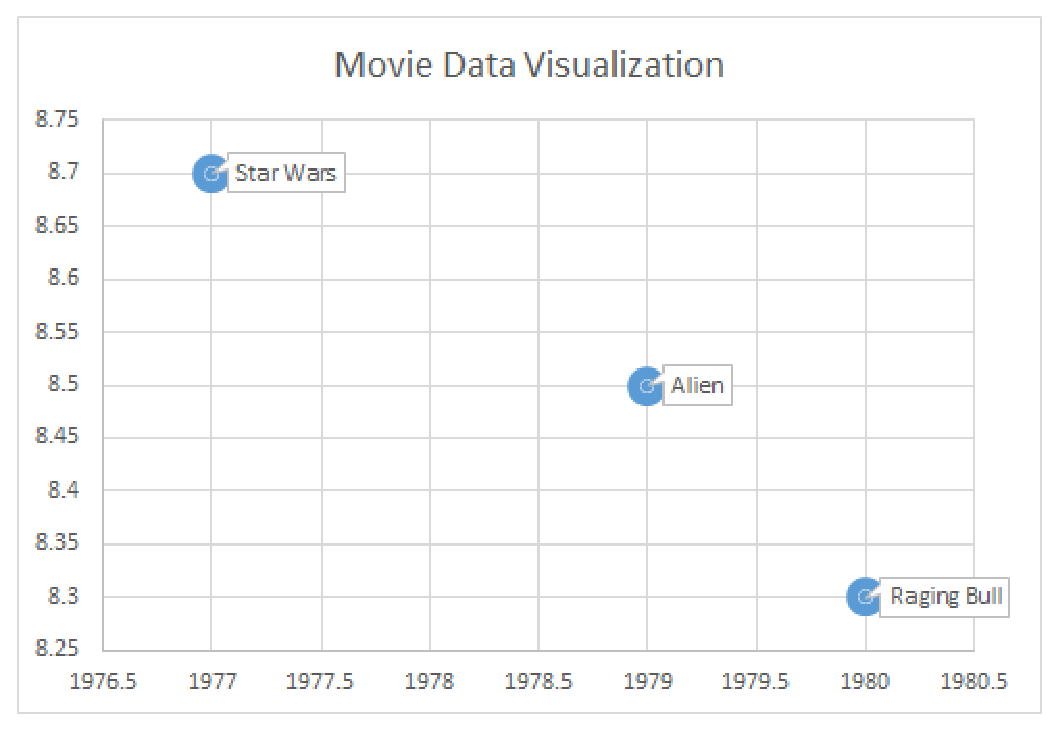
\includegraphics[width=\linewidth]{images/ExampleVisualEncoding.eps}
  \caption{\label{fig:ExampleVisualEncoding}%
           An example visual encoding for movie-data. }
\end{figure}

